\documentclass[11pt, a4paper]{article}

% --- ESSENTIAL PACKAGES ---

% Font Encoding and Input
\usepackage[T1]{fontenc} % Use 8-bit T1 fonts to ensure proper character rendering
\usepackage[utf8]{inputenc} % Allows direct use of UTF-8 characters (e.g., é, ö, à)
\usepackage{amsmath} % For \text{} in math mode

% Page Layout and Margins
\usepackage{geometry}
\geometry{
    a4paper,
    left=2.5cm,
    right=2.5cm,
    top=3cm,
    bottom=3cm
}

% Professional Fonts (Latin Modern)
\usepackage{lmodern}
\usepackage{helvet} % For Helvetica font, used for the main title

% --- COLOR AND STYLING ---

% Color Management
\usepackage[dvipsnames]{xcolor} % Use dvipsnames for a wider range of predefined colors

% Define a professional color palette
\definecolor{primary}{HTML}{0A369D}  % A deep, professional blue
\definecolor{secondary}{HTML}{4472CA} % A lighter, complementary blue
\definecolor{darkgray}{HTML}{333333}  % For body text, better than pure black
\definecolor{customgreen}{HTML}{5E8B7E} % A muted green for accents
\definecolor{titleblue}{HTML}{082A75} % A darker, rich blue for the main title

\color{darkgray} % Set the default text color

% Section and Title Styling
\usepackage{titlesec}
\titleformat{\section}
  {\normalfont\Large\bfseries\color{primary}} % Format for the section title
  {\thesection}{1em}{} % Section number, spacing, and the title itself
\titleformat{\subsection}
  {\normalfont\large\bfseries\color{secondary}}
  {\thesubsection}{1em}{}
\titleformat{\subsubsection}
  {\normalfont\bfseries\color{customgreen}}
  {\thesubsubsection}{1em}{}

% --- IMAGES AND GRAPHICS ---

% Standard package for including images
\usepackage{graphicx}
\graphicspath{{images/}} % Optional: specify a folder for your images
\usepackage{float} % Improved control over figure placement with [H] option

% --- LISTS AND ENUMERATIONS ---

% Customize list environments
\usepackage{enumitem}
% The 'textcolor' option sets the color for the item's text
\setlist[itemize,1]{label=\textcolor{primary}{\textbullet}}
\setlist[itemize,2]{label=\textcolor{secondary}{\textendash}}

% --- HYPERLINKS ---

% Hyperlink styling for URLs and cross-references
\usepackage{hyperref}
\hypersetup{
    colorlinks=true,
    linkcolor=primary,
    filecolor=magenta,
    urlcolor=secondary,
    citecolor=customgreen,
    pdftitle={My Professional Document},
    pdfpagemode=FullScreen,
}

% --- TYPOGRAPHY AND MICRO-ADJUSTMENTS ---

% Improves the justification and spacing of text for a cleaner look
\usepackage{microtype}

% --- DOCUMENT CONTENT EXAMPLE ---

% For placeholder text
\usepackage{lipsum}

% --- TABLE AND CURRENCY PACKAGES ---
\usepackage{booktabs} % For professional looking tables
\usepackage{longtable} % For tables that may span multiple pages
\usepackage{siunitx} % For aligning numbers in tables
\usepackage{eurosym} % For the EUR symbol
\usepackage{float} % to use [H]
\usepackage{ragged2e}

% --- GLOSSARIES ---
\usepackage[acronym]{glossaries}
\makeglossaries

\newacronym{genai}{GenAI}{Generative AI}
\newacronym{pca}{PCa}{Prostate Cancer}
\newacronym{njde}{NJDE}{Neural Jump Ordinary Differential Equation}
\newacronym{mri}{MRI}{Magnetic Resonance Imaging}
\newacronym{pet}{PET}{Positron Emission Tomography}
\newacronym{ct}{CT}{Computed Tomography}
\newacronym{ehr}{EHR}{Electronic Health Record}
\newacronym{vae}{VAE}{Variational Autoencoder}
\newacronym{trl}{TRL}{Technology Readiness Level}
\newacronym{psma}{PSMA}{Prostate-Specific Membrane Antigen}
\newacronym{ttp}{TTP}{Time-to-Progression}
\newacronym{eau}{EAU}{European Association of Urology}
\newacronym{wsi}{WSI}{Whole-Slide Images}
\newacronym{tcga}{TCGA-PRAD}{The Cancer Genome Atlas - Prostate Adenocarcinoma}
\newacronym{eucaim}{EUCAIM}{European Cancer Imaging Initiative}
\newacronym{sla}{SLA}{Service Level Agreement}
\newacronym{cdm}{CDM}{Common Data Model}
\newacronym{omopcdm}{OMOP-CDM}{Observational Medical Outcomes Partnership - Common Data Model}
\newacronym{fhir}{HL7 FHIR}{Health Level Seven - Fast Healthcare Interoperability Resources}
\newacronym{dsa}{DSA}{Data Sharing Agreement}
\newacronym{gdpr}{GDPR}{General Data Protection Regulation}
\newacronym{fid}{FID}{Fréchet Inception Distance}
\newacronym{ssim}{SSIM}{Structural Similarity Index Measure}
\newacronym{lpips}{LPIPS}{Learned Perceptual Image Patch Similarity}
\newacronym{auc}{AUC}{Area Under the Curve}
\newacronym{mae}{MAE}{Mean Absolute Error}
\newacronym{cindex}{C-index}{Concordance Index}
\newacronym{ood}{OOD}{Out-of-Distribution}
\newacronym{xai}{XAI}{eXplainable AI}
\newacronym{eibir}{EIBIR}{European Institute for Biomedical Imaging Research}
\newacronym{dicom}{DICOM}{Digital Imaging and Communications in Medicine}
\newacronym{adt}{ADT}{Androgen Deprivation Therapy}
\newacronym{ap}{AP}{Alkaline Phosphatase}
\newacronym{asap}{ASAP}{Atypical Small Acinar Proliferation}
\newacronym{bcr}{BCR}{Biochemical Recurrence}
\newacronym{bph}{BPH}{Benign Prostatic Hyperplasia}
\newacronym{crpc}{CRPC}{Castration-Resistant Prostate Cancer}
\newacronym{ctc}{CTCs}{Circulating Tumor Cells}
\newacronym{ece}{ECE}{Extracapsular Extension}
\newacronym{ene}{ENE}{Extranodal Extension}
\newacronym{hgpin}{HGPIN}{High-Grade Prostatic Intraepithelial Neoplasia}
\newacronym{lvi}{LVI}{Lymphovascular Invasion}
\newacronym{psadt}{PSADT}{PSA Doubling Time}


\title{A Causal AI Framework for Longitudinal Modelling of Prostate Cancer}
\author{}
\date{}

\begin{document}

\maketitle

\begin{abstract}
This project introduces a new paradigm in oncology with an interactive, Generative AI (GenAI)-based agent for managing prostate cancer (PCa). We will build a causal "digital twin" to transparently model the disease trajectory by integrating complex multimodal data into a unified patient view. Technologically, we will fuse multimodal data, use GenAI for data augmentation, and create a medical knowledge base by disentangling disease signals from confounders. Clinically, our agent will improve diagnosis by simulating disease progression and enable personalized treatment selection by forecasting outcomes. The framework is designed as a trustworthy, explainable, and safe AI system compliant with the EU AI Act, establishing a new European standard for medical GenAI.
\end{abstract}

\section{Excellence}

\subsection{Objectives and Relevance to the Challenge}
The project's objectives are designed to be SMART and are explicitly aligned with the specific objectives of the EIC Pathfinder Challenge: \textbf{Generative-AI based Agents to Revolutionize Medical Diagnosis and Treatment of Cancer}. Our proposal for \gls{pca} addresses both the technological and clinical areas of the challenge.

\subsubsection*{Area 1: Technological Area}
\begin{itemize}
    \item \textbf{\gls{genai}-based tools for Integrating Multidimensional Multimodal Health Data (i):} We will develop and validate a novel Causal AI framework, built upon a \gls{njde} architecture. This model will pioneer the integration of multidimensional and multimodal data—including imaging (\gls{mri}, \gls{pet}, \gls{ct}), \gls{ehr}, pathology, and -omics data—into a unified, dynamic patient model. This foundational technology will establish a new European standard for clinical AI. A key technical objective is to master data heterogeneity through a robust \gls{vae} framework that disentangles true disease signals from confounders, ensuring the model is robust and generalizable across diverse European healthcare systems.

    \item \textbf{Medical Data Augmentation through Counterfactual and Cross-Modality Synthesis (ii):} Our framework will employ advanced \gls{genai} techniques for two key data augmentation purposes. Firstly, we will generate \textbf{counterfactual images} to enrich the dataset with controlled variations. For example, we can synthesize how a specific patient's scan might look at a different age or an earlier/later stage of the disease. This allows the model to learn the specific visual impact of these factors. Secondly, we will perform \textbf{cross-modality synthesis} (e.g., generating a synthetic \gls{ct} from an existing \gls{mri}) not for a single application, but to create more complete data pairs. This capability addresses the common clinical problem of missing modalities, enabling more robust, multi-modal model training and accelerating research and development across the EIC portfolio.

    \item \textbf{Medical Knowledge Integration via Strong Inductive Biases (iii):} Our framework moves beyond simplistic "black-box" models by creating a comprehensive medical knowledge base, not as a separate component, but by deeply embedding extensive domain knowledge directly into the model's architecture and training process. This is achieved through a multi-layered strategy of applying strong, clinically-informed inductive biases:
    \begin{itemize}
        \item \textbf{At the Feature Level:} We will incorporate prognostic features explicitly recommended by urological guidelines, such as \gls{psadt} and tumor volume, directly into the model's input, ensuring it is grounded in established clinical practice.
        \item \textbf{At the Architectural Level:} The core of our knowledge integration lies in the principled disentanglement of the \gls{vae}'s latent space. By architecturally separating anatomy from disease to the extent that it is not harmful, we impose a strong prior that a tumor should not fundamentally alter a patient's pelvic bone structure, a powerful form of embedded domain knowledge.
        \item \textbf{At the Objective Level:} We will use specialized, knowledge-infused loss functions. For ordinal variables like Gleason Grade or PI-RADS scores, a \textbf{differential ordinal loss} ensures the model understands their inherent ranking and severity progression, a concept a standard classification loss ignores.
        \item \textbf{At the Training Strategy Level:} The temporal model (\gls{njde}) will be pre-trained on a simplified, rule-based decision algorithm derived directly from established \textbf{\gls{eau} clinical guidelines}. This provides the model with a robust, clinically-valid starting point for understanding disease progression before fine-tuning on complex real-world data.
    \end{itemize}
    This multi-faceted infusion of domain knowledge ensures the model learns the true underlying causal mechanisms of the disease. The resulting clinically plausible, visual counterfactuals are a direct output of this knowledge-grounded architecture, enabling clinicians to ask meaningful "what-if" questions and receive intuitive, reliable explanations. Robust methods for uncertainty quantification will also be integrated to reliably flag high-uncertainty cases for human review.
\end{itemize}

\subsubsection*{Area 2: Clinical Area}
\begin{itemize}
    \item \textbf{Predictive Diagnosis and In-Silico Trials (i):} We will develop an interactive agent capable of providing a personalized, dynamic prognosis. The agent will simulate a patient's future disease trajectory, generating predictions of not only future scans but also key, validated clinical endpoints such as future \textbf{TNM stage, PI-RADS scores}, and the likelihood of \textbf{\gls{bcr}}. This provides a comprehensive prognostic tool to improve diagnostic precision and risk stratification, reducing over- and under-treatment. Furthermore, this simulation capability transforms the model into a powerful platform for \textit{in-silico} clinical trials. By modeling counterfactual patient journeys under different diagnostic or therapeutic assumptions, we can generate and pre-test robust research hypotheses, allowing for the design of more targeted, efficient, and ethical human clinical trials in the future.

    \item \textbf{Enhance Personalized Treatment Selection (ii):} We will deliver a treatment-choice helper that, while respecting the \textbf{\gls{eau} guidelines} as the gold standard, directly addresses their acknowledged evidence gaps. The agent will leverage the "digital twin" to forecast outcomes for different treatment pathways, optimizing for maximum \gls{ttp}. Critically, this will help resolve uncertainty around the use of \textbf{\gls{psma} \gls{pet}/\gls{ct}}. While its high sensitivity for early disease detection is known, a lack of extensive clinical trial data means guidelines cannot yet specify how to best act on this information. Our model will generate evidence by simulating outcomes, helping to form hypotheses for how \gls{psma} \gls{pet}/\gls{ct} findings can be optimally integrated into treatment decisions. Furthermore, our project will create one of Europe's most comprehensive datasets on \textbf{$^{177}$Lu-\gls{psma} therapy}, a novel and highly promising treatment. By modeling this rich data, we aim to significantly improve the utilization of this therapy, identifying the patient subgroups who will benefit most and the optimal timing for its administration.
\end{itemize}

\subsection{Novelty: A Paradigm Shift from Prediction to Causal Understanding}
The management of \gls{pca} is complex, with risks of overdiagnosis and undertreatment. The disease's natural history is a multi-stage process influenced by tumor biology, patient characteristics, and interventions. This project proposes a paradigm shift from prediction to deep causal reasoning. We will build a dynamic, interactive "digital twin" of a patient’s disease trajectory that (i) encodes heterogeneity, (ii) learns cause-and-effect mechanisms, and (iii) simulates future trajectories, updating predictions with new data.

Under treatment, tumors can evolve, leading to uncertainty about when to switch therapy. The expanding options, including targeted agents and advanced imaging, add to this complexity. Clinical guidelines use discrete risk categories, but the disease is a continuous process. Our model is designed to capture this patient-specific trajectory, offering a personalized assessment.

This complex, multi-stage evolution is visualized in Figure \ref{fig:prostate_evolution}. It illustrates how a combination of imaging, lab studies, and clinical findings are needed to understand where a patient is on their disease timeline. A key novelty of our project is the explicit modeling of this temporal dimension. By integrating all measurements across the entire patient journey, we can build a dynamic understanding of disease progression, which is a significant leap beyond current static assessments.

\begin{figure}[H]
    \centering
    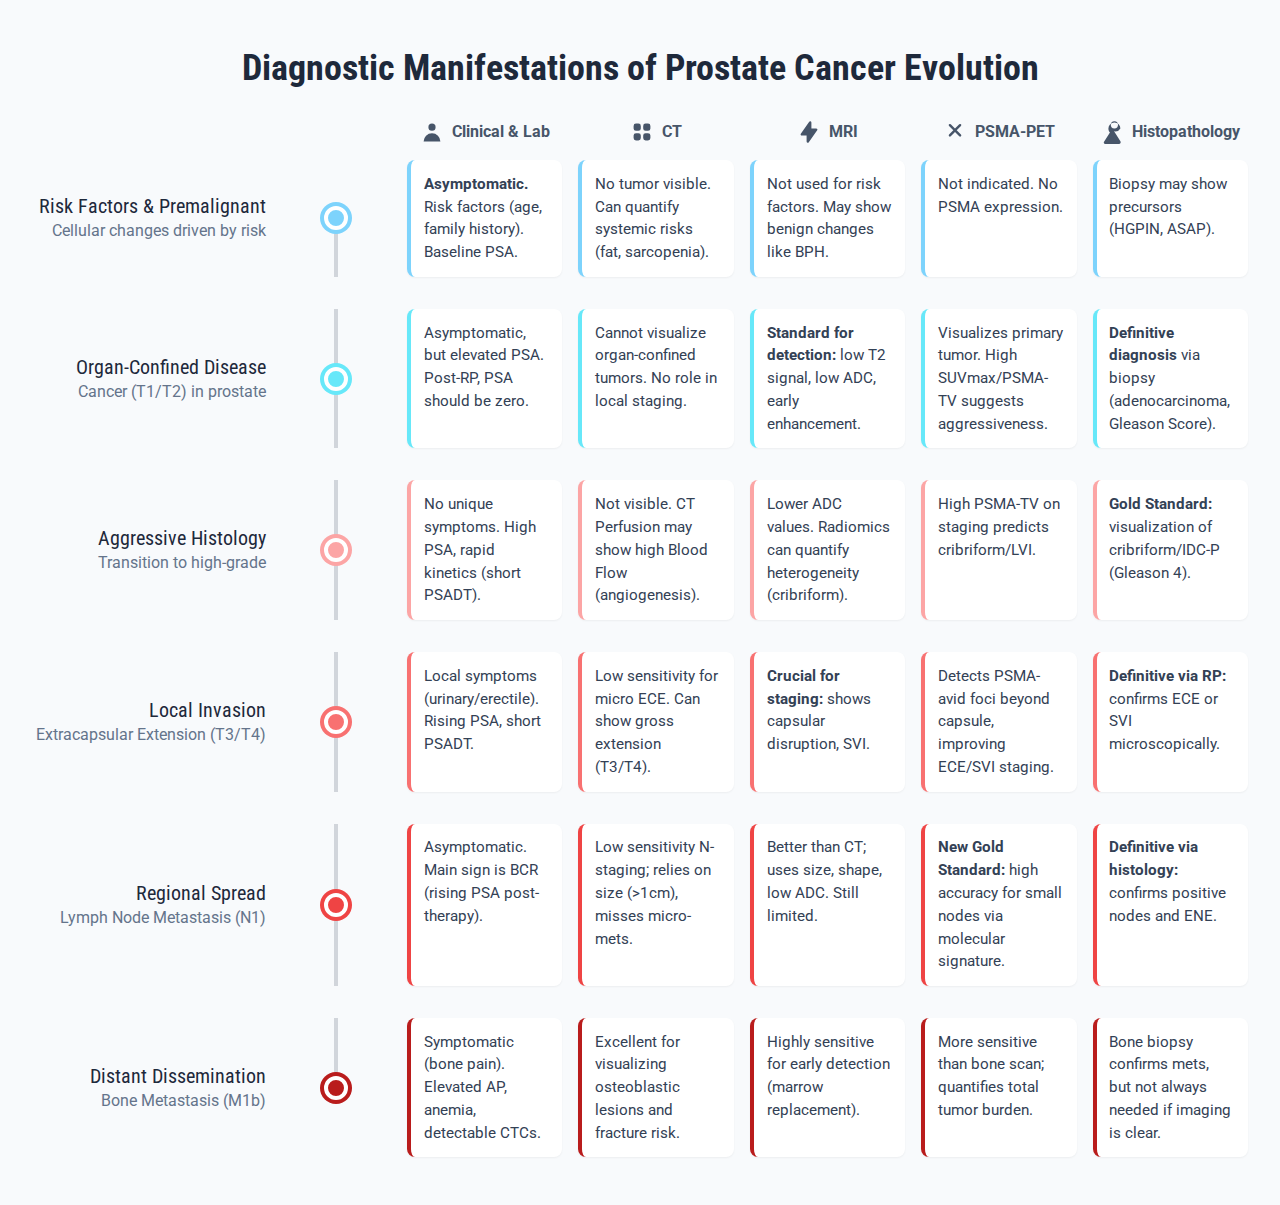
\includegraphics[width=\textwidth]{pe.png}
    \caption{The natural history of prostate cancer, illustrating the stages our model will learn. The disease evolves based on tumor stage, patient state, and interventions, with information inferred from multiple clinical and imaging modalities. Our hypothesis is moreover that stage of a disease at initial diagnosis is the key to the best futher theraphy \textbf{Abbreviations:} \gls{adt}, \gls{ap}, \gls{asap}, \gls{bcr}, \gls{bph}, \gls{crpc}, \gls{ctc}, \gls{ece}, \gls{ene}, \gls{hgpin}, \gls{lvi}, \gls{psadt}}
    \label{fig:prostate_evolution}
\end{figure}

\paragraph{What is Radically New: A Comprehensive Framework for Causal Learning.}
The core technical innovation of this project is a \textbf{single, comprehensive framework} that makes large-scale causal learning on complex 3D medical data feasible for the first time. While Neural Ordinary Differential Equations (NODEs) are powerful for modeling continuous processes, their application to high-dimensional 3D data has been largely intractable due to prohibitive computational costs. Our radical solution is to apply the NODE not to the raw data, but to a carefully constructed, low-dimensional \textbf{disentangled latent space}. This innovation is what makes the entire framework possible.

This is not just a dimensional reduction trick; it is a new paradigm for building knowledge-grounded models. We combine this latent-space dynamic modeling with several other cutting-edge techniques in a completely new way:
\begin{itemize}
    \item \textbf{Neural Jump ODEs:} We explicitly model the reality of clinical care by treating disease progression as a continuous process (the ODE) punctuated by radical, discrete interventions like surgery or therapy (the "jumps").
    \item \textbf{Loss Masking:} We overcome the challenge of sparse, real-world clinical data by using a masked loss function, allowing the model to learn from incomplete time series without being penalized for missingness.
    \item \textbf{Deep Domain Knowledge Integration:} Our model is not a black box; it is infused with medical knowledge at every level. We use ordinal losses to respect the clinical severity of scales like PI-RADS, pre-train the temporal model on established EAU guidelines, and architecturally separate anatomical factors from disease signals.
\end{itemize}

By creatively fusing these technologies, we are creating a single, unified pipeline that can accelerate clinical work by auto-generating radiological reports, enhance prediction by modeling the entire patient journey, and enable rapid, low-cost experimentation of new clinical hypotheses. This project forges the technology-to-come: a foundational causal framework that integrates multi-scale evidence into robust, updatable decision processes, establishing a new European reference architecture for trustworthy, explainable, and regulation-ready medical AI.

\subsection{Plausibility of the Methodology: A Feasible Path to a Groundbreaking Technology}
Our methodology is a direct answer to the profound challenges of building trustworthy clinical AI. We aim to design a novel, \textbf{four-stage causal framework} that deconstructs the immense complexity of prostate cancer progression into a series of well-defined, manageable tasks. This modular approach is the key to our project's feasibility: it ensures training stability, enhances model interpretability, and allows us to systematically embed clinical domain knowledge as strong inductive biases. This extensive integration of domain knowledge is crucial for ensuring the model generalizes well beyond its training data. The use of a carefully crafted disentangled latent space is a direct and innovative response to the "curse of dimensionality"; without this approach, reliably training a model on such complex, time-varied, and incomplete data would be practically impossible. Each element of our proposed framework is based on strong, peer-reviewed research, ensuring that our ambitious goals are built on a solid scientific foundation. This guides the model to learn the true underlying causal mechanisms of the disease, rather than superficial correlations.

This project will start at a Technology Readiness Level (TRL) of 1 for the general framework, as it involves fundamental research into a new causal AI paradigm. However, for the initial data processing and management components, we will begin at TRL 3. This is possible because we will leverage and build upon the tools and infrastructure developed in a different, but highly relevant, project: \textbf{SIKIT: Strengthening Autonomy in the Implementation of AI Technologies in Medicine}. SIKIT is a major interdisciplinary project with \textbf{total funding of €1,290,924.68} from the "Sachsen-Anhalt WISSENSCHAFT" program (co-financed by the EU's EFRE program), running for \textbf{42 months (July 2024 - December 2027)}. This existing foundation provides a significant head start and de-risks the initial phases of our proposed project.

This design leverages the project team's extensive experience in synthetic image generation (\gls{ct} from \gls{pet}) and predictive modeling, and is illustrated in Figure \ref{fig:ml_framework}. The proposed framework will address the current limitations in clinical guidelines, particularly the uncertainty surrounding the integration of new imaging modalities like \gls{psma}-\gls{pet}. By creating a digital model of the patient and the disease, our system will be able to simulate virtual interventions and generate research hypotheses. This capability will be crucial for designing targeted and efficient clinical trials to establish how to best use new diagnostic information, ultimately saving time, money, and reducing patient risk.


\subsubsection{Stage 1: Building the Bedrock of Clinical Validity with Supervisor Models}
The first stage builds a suite of specialized "supervisor" models. These models act as expert guides, providing strong, clinically-validated signals that will enforce a valid structure on the more complex generative models in subsequent stages. Our team's prior success in developing predictive models from fused clinical and imaging data provides a strong foundation for this work package.
\begin{itemize}
    \item \textbf{Ordinal Classifiers:} For clinical scores with an inherent order (e.g., PI-RADS, TNM stage), standard categorical classifiers are suboptimal. We will implement a \textbf{differential ordinal learning framework} that explicitly encodes the ordered structure by combining a standard categorical loss with a differential ordinal loss, ensuring the model understands that a higher grade implies a worse prognosis \cite{LeeByeon2025, GrisiKartasalo2025}.
    \item \textbf{Censored Survival Regressor:} To predict \gls{ttp}, we will train a survival model that properly handles right-censored data. This will be achieved using a censored regression loss (e.g., Logistic Hazard) combined with a ranking loss regularizer (e.g., SurvRNC) to ensure correct risk ordering in the learned feature representation \cite{GaoLi2019, RivailVogl2023, SaeedRidzuan2024}.
This approach ensures the model generalizes well and produces more clinically plausible counterfactuals \cite{PuglisiAlexander2025, ZhangHager2025}.
\end{itemize}

\subsubsection{Stage 2: Mastering Heterogeneity through Principled Disentanglement}
At the heart of our solution to data heterogeneity is a hierarchical \gls{vae} trained for each imaging modality to learn a disentangled latent space. The key innovation is partitioning this space into four independent, semantically meaningful components: Anatomy ($Z_A$), Disease ($Z_D$), Patient State ($Z_P$), and Style/Confounders ($Z_S$). This separation is enforced through a composite loss function:
$$ \mathcal{L}_{\text{total}} = \mathcal{L}_{\text{VAE}} + \lambda_A \mathcal{L}_{\text{Anatomy}} + \lambda_D \mathcal{L}_{\text{Disease}} + \lambda_I \mathcal{L}_{\text{Disentangle}} $$
The disentanglement is achieved by moving beyond simple $\beta$-VAE approaches. Our loss function will apply a \textbf{targeted penalization} of the statistical dependence between latent subspaces. We recognize that some correlations are clinically meaningful (e.g., disease can affect anatomy), while others are spurious. Therefore, the model will be heavily penalized for mutual information between causally independent subspaces (e.g., Disease $Z_D$ and Style $Z_S$, which includes scanner type and data source), while allowing for natural correlations between dependent factors like disease and anatomy. This is accomplished by selectively applying a Total Correlation (TC) penalty, ensuring the learned disease representation is invariant to technical artifacts without sacrificing the reconstruction of clinically valid relationships \cite{FragemannArdizzone2022, AbbasiMonadjemi2018, FayCobos2023}. The entire data curation and preprocessing pipeline is visualized in Figure \ref{fig:data_curation}.

\begin{figure}[H]
    \centering
    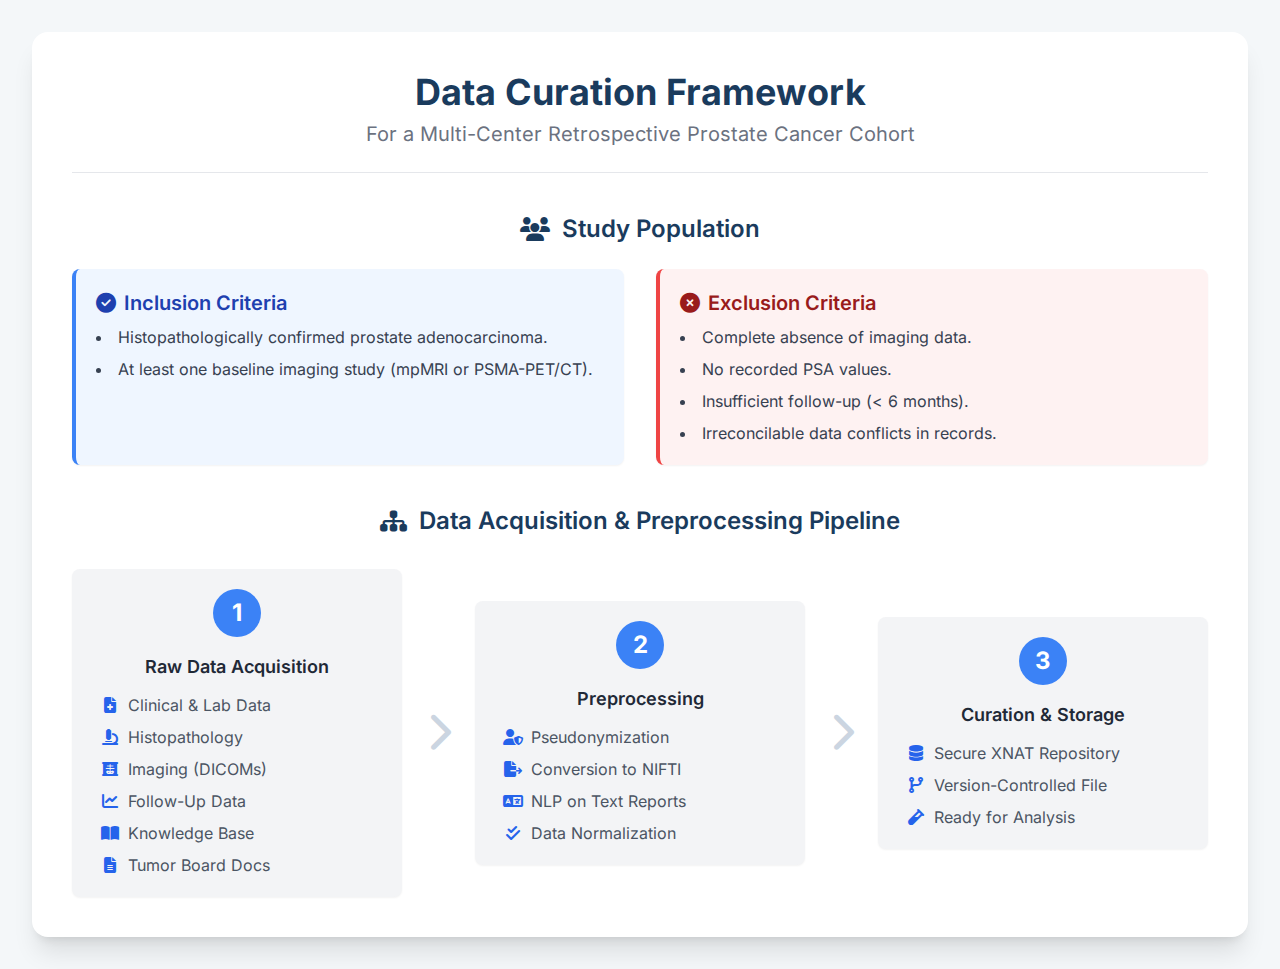
\includegraphics[width=\textwidth]{dc.png}
    \caption{An infographic summarizing the data acquisition, curation, and preprocessing framework for the study cohort. It details the inclusion and exclusion criteria for patient selection and outlines the multi-step pipeline for processing clinical, histopathological, and imaging data. The \gls{ehr} is a key source of clinical data.}
    \label{fig:data_curation}
\end{figure}

\subsubsection{Stage 3: Capturing Disease Dynamics with Neural Jump ODEs}
This stage confronts the critical challenge of modeling disease evolution from sparse, multimodal, and irregularly-sampled clinical data. Our solution is a \textbf{\gls{njde}} framework, which is uniquely suited for this task \cite{GwakSim2020}.

\paragraph{Rationale and Latent State Formulation}
Neural Ordinary Differential Equations (NODEs) are powerful because they model system dynamics in continuous time, making them inherently robust to irregular sampling—a defining characteristic of clinical data \cite{GwakSim2020, JohnsonBulgarelli2023, BelogolovskyGreenberg2023}. However, their primary weakness is the extreme computational cost of applying them directly to high-dimensional data like 3D images \cite{WiewelBecher2018, DavisChoromanski2020}. Our approach strategically mitigates this by operating exclusively on the low-dimensional latent spaces learned in Stage 2. This is not just an efficiency gain; thanks to the successful disentanglement, we do not need to pass the entire latent space to the temporal model. Instead, by training the NODE only on the most relevant parts—the disentangled \textbf{disease ($Z_D$) and patient state ($Z_P$) components}—we focus the model on learning the dynamics of disease progression itself, making the learning task more tractable and clinically relevant \cite{AshmanSo2020, KberKalisch2023, LosadaTerranova2024}. Crucially, by modeling the evolution of these purified latent vectors, we are not just fitting a curve to data points; we are learning a representation of the underlying causal trajectory of the disease, stripped of observational noise and technical artifacts.

The input for the \gls{njde} is a carefully constructed time series of latent state vectors. For each patient, we define a unified state vector $\mathbf{v}$ that has a fixed shape, representing a concatenation of all possible inputs. The process is as follows:
\begin{enumerate}
    \item \textbf{Unified State Vector Definition:} A canonical tensor shape is defined for a state vector $\mathbf{v}$, which includes dedicated slots for the disease latent code ($Z_D$) and patient state code ($Z_P$) from each imaging modality (\gls{mri}, \gls{pet}, SPECT), and for embeddings of all non-imaging data (PSA, clinical note embeddings, etc.).
    \item \textbf{Time-stamped Sparse Tensor Creation:} For each time point $t_i$ where a patient has data, a new state vector $\mathbf{v}(t_i)$ is created and initialized with zeros. The available data is then placed into its corresponding slot in the tensor. For example, at a time point with a \gls{pet} scan and PSA value, only the $Z_{D_{\text{PET}}}$, $Z_{P_{\text{PET}}}$, and PSA embedding slots are filled, while all other slots remain zero.
    \item \textbf{Anatomy Vector Storage:} The patient-specific anatomy vectors ($Z_A$) from each imaging study are not included in the dynamic state vector but are stored separately, indexed by time, for use in the final image reconstruction stage.
\end{enumerate}
This procedure yields a dataset of sparse, irregularly-sampled latent state vectors, providing a computationally efficient and robust representation of each patient's unique clinical history.

\paragraph{NJDE Training and Dynamics}
The \gls{njde} learns the rules of disease evolution by modeling two phenomena \cite{GwakSim2020}:
\begin{itemize}
    \item \textbf{Continuous Evolution (The NODE):} Between clinical events, the disease state evolves smoothly. This is modeled by a classic NODE that learns the underlying dynamics from the sparse state vectors \cite{BergHasenclever2018}.
    $$ \frac{d\mathbf{v}(t)}{dt} = f(\mathbf{v}(t), t; \psi) \quad \text{for } t \neq t_k $$
    \item \textbf{Discrete Jumps (The Interventions):} At the specific time $t_k$ of a clinical intervention (e.g., radical prostatectomy, initiation of systemic therapies such as \gls{adt} or chemotherapy, or targeted radioligand therapy with $^{\text{177}}\text{Lu-PSMA}$), the continuous evolution is interrupted by a discrete "jump." A separate neural network, $g$, models this instantaneous change to the state vector based on the type of intervention \cite{CuchieroLarsson2019, AbushaqraXue2022}. Crucially, the model is designed to handle multiple, sequential jumps, allowing it to accurately represent a patient's entire treatment history, which may involve several different lines of therapy over time.
    $$ \mathbf{v}^+ = g(\mathbf{v}(t_k), \text{intervention}_k; \phi) \quad \text{for } t = t_k $$
\end{itemize}


\begin{figure}[H]
    \centering
    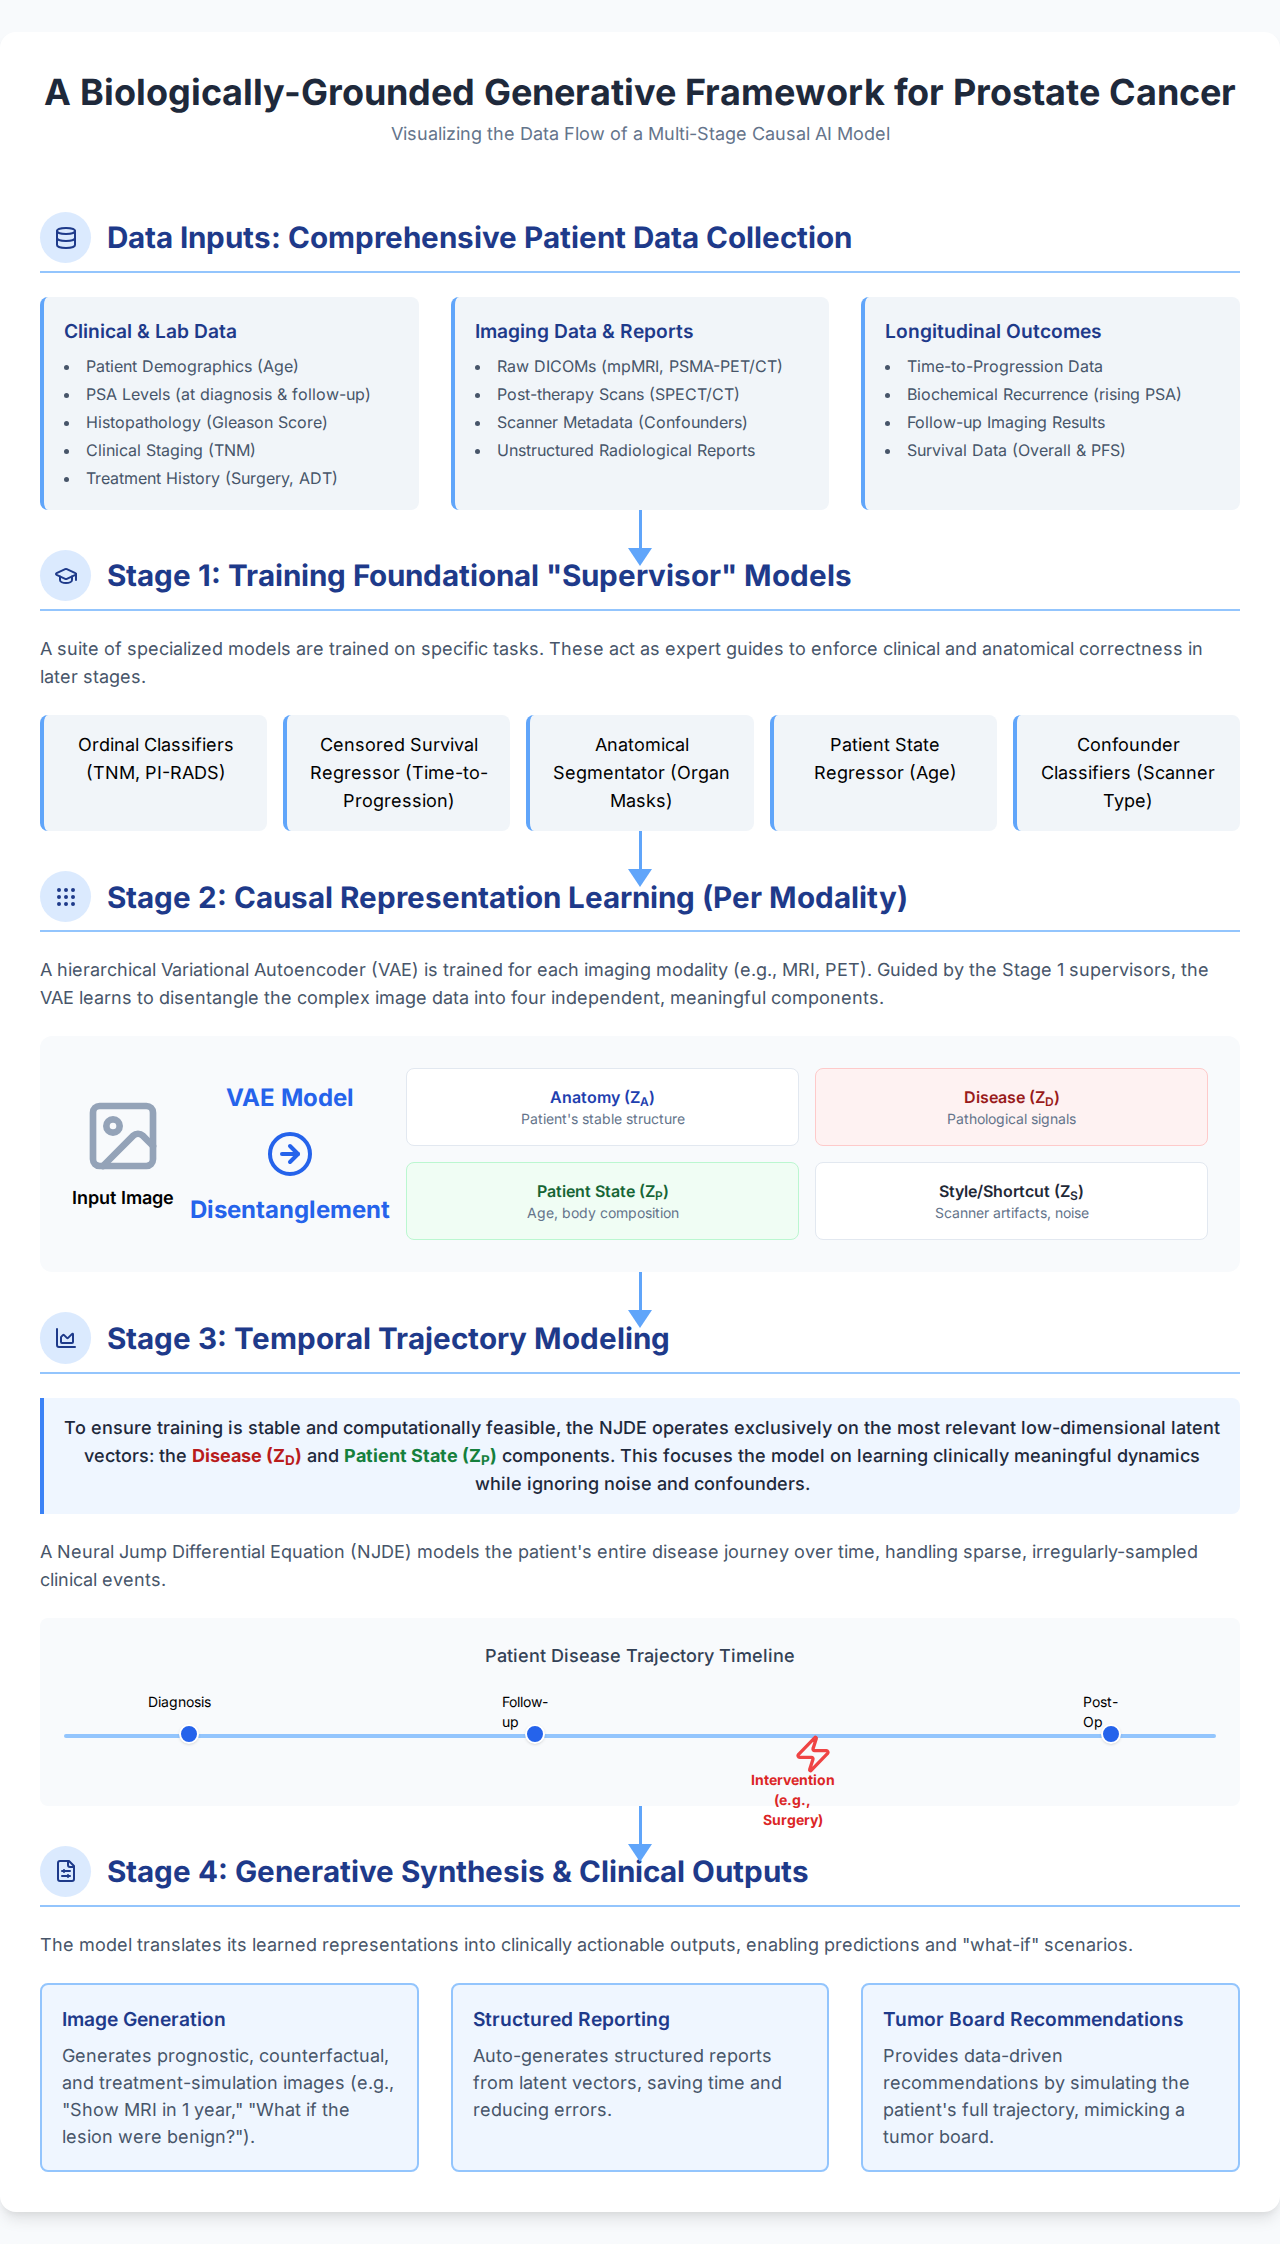
\includegraphics[        trim=5mm 30mm 5mm 20mm, % {left bottom right top}
        clip,                     % This command applies the trim
        width=\textwidth]{ml.png}
    \caption{The proposed multi-stage causal AI framework.}
    \label{fig:ml_framework}
\end{figure}

This hybrid approach, which explicitly separates the continuous disease course from the rapid, external impacts of clinical interventions, is critical for accurately modeling a patient's journey \cite{GwakSim2020}. The model is trained using a \textbf{leave-one-out strategy} for each patient's time series: given all but one time point, its goal is to predict the complete state vector for the held-out time point. To handle the pervasive missing data, we will first develop a simplified, rule-based decision algorithm in close consultation with our urology partners. This algorithm, based on the \gls{eau} guidelines, will provide a baseline management recommendation even for cases with incomplete data. The \gls{njde} model will then be pre-trained on the outputs of this decision tree, allowing it to develop an initial, robust understanding of the relationships between patient state, disease status, and appropriate management pathways before being fine-tuned on the full, complex tumour board data. For the fine-tuning stage, we will employ a \textbf{masked loss function}. The loss is calculated only by comparing the predicted values to the ground truth for those elements of the state vector that were actually available (non-zero) at the target time point. This forces the model to learn a probable evolution for every data type, even from a highly incomplete dataset. By distinguishing between smooth progression and intervention-driven shocks, the \gls{njde} learns a more biologically plausible model of the patient's journey.

\subsubsection{Stage 4: Translating Insight into Action: Generative Synthesis, Decision Support, and Structured Reporting}
The final stage translates the model's learned causal dynamics into clinically actionable outputs, evolving the framework from a descriptive tool into an active partner in clinical decision-making. This includes generating high-fidelity images for any time point or counterfactual scenario, with a lightweight Diffusion Model used as a final post-processing step to ensure realism. These visual outputs serve as the intuitive foundation for the system's core decision support capabilities.

A key innovation in this stage is the use of clinician interaction patterns as a feedback loop. The framework's user interface will be designed to log all interactions, such as the specific "what-if" questions asked, the counterfactuals generated, and the treatment scenarios explored by the clinician. This interaction data will be analyzed to identify recurring patterns of inquiry, which can provide valuable insights into the clinician's diagnostic and treatment-planning thought process. This information will then be used to personalize the "digital twin's" outputs in two ways:
\begin{itemize}
    \item \textbf{Personalized Explanations:} By understanding the questions a clinician frequently asks about a particular type of case, the system can proactively generate the most relevant counterfactuals and visualizations, tailoring its explanations to the user's specific cognitive workflow.
    \item \textbf{Adaptive Patient-Facing Visualizations:} The system will use the insights from clinician interactions to create simplified, more intuitive visualizations of the expected disease progression for patients. By knowing what aspects of the data are most critical for decision-making, the system can generate clearer, more focused graphical timelines and outcome predictions, helping patients to better understand their condition and treatment options.
\end{itemize}

Crucially, the framework will function as a \textbf{Treatment-Choice Helper}. Leveraging the \gls{njde} from Stage 3, the system will simulate multiple future patient trajectories, each conditioned on a different potential treatment intervention and timing. By comparing these simulated outcomes, the model can identify the therapeutic strategy that is explicitly optimized to \textbf{maximize the expected time to progression}. This transforms the "what-if" capability from a simple explanatory tool into a powerful engine for data-driven treatment planning.

All insights are then consolidated into automatically generated structured reports using a \textbf{Transformer-based decoder}. These reports will integrate prognostic simulations, present the comparative effectiveness of different treatment options, and culminate in a data-driven recommendation. This directly addresses the clinical need for clear, consistent, and efficient documentation \cite{JorgHalfmann2023, SacoranskyKwan2024}, while providing clinicians with novel, data-driven strategies for patient management. The project team's experience in creating LLM-based support apps and GUIs from structured reports is key to ensuring this complex information is presented in an intuitive and actionable format.

\section{Impact}
This project will generate significant and lasting impact by advancing the frontiers of science and technology and delivering tangible benefits to patients, clinicians, and the European innovation ecosystem. We aim to establish a new technological paradigm for clinical AI that is trustworthy, explainable, and aligned with the goals of the EU Cancer Mission.

\subsection{Potential Impact: Pathways to Outcomes}
\begin{itemize}
    \item \textbf{Enhanced Diagnostic Accuracy and Personalised Treatment:} Enable more accurate staging, better risk stratification, and personalized treatment planning, reducing over- and under-treatment.
    \item \textbf{Empowering Clinicians and Reducing Workload:} Augment clinical decision-making and reduce documentation time with intuitive explanations and automated structured reports.
    \item \textbf{A Foundation for a New Era in European Oncology:} Provide a disease-agnostic foundational technology adaptable to other cancers and chronic diseases.
\end{itemize}

\subsection{Innovation Potential}
\begin{itemize}
    \item \textbf{A New European Standard for Trustworthy Clinical AI:} Pioneer a shift from "black-box" models to causal AI, establishing a new European standard for trustworthy AI in high-stakes environments.
    \item \textbf{Advancing the Frontier of Generative AI:} Push the boundaries of generative AI with novel techniques in disentanglement, counterfactual generation, and longitudinal modeling.
    \item \textbf{Fostering an Open and Sovereign European AI Ecosystem:} Make all code open-source and contribute curated, anonymized datasets to the \gls{eucaim} platform.
\end{itemize}

\subsection{Communication, Dissemination, and Exploitation}
\begin{itemize}
    \item \textbf{High-Impact Scientific Publications:} Target leading peer-reviewed journals and present findings at premier international conferences.
    \item \textbf{Open Source and Open Data:} All code will be open-sourced, and curated, anonymized datasets will be contributed to the \gls{eucaim} platform.
    \item \textbf{Engagement with Clinical and Patient Community:} Actively engage with European clinical societies and patient advocacy groups to ensure clinical relevance and facilitate translation.
    \item \textbf{Commercial Exploitation and Standardization:} Explore commercialization through partnerships with industry leaders and participate in standardization bodies to promote adoption.
\end{itemize}

\section{Implementation}

\subsection{Work Plan and Risk Mitigation}
The project is structured into eight interconnected Work Packages (WPs) over a 36-month duration, as visualized in the Gantt chart (Figure~\ref{fig:gantt}). A detailed risk analysis and mitigation strategy is provided in Table \ref{tab:risks}.

\begin{figure}[H]
    \centering
    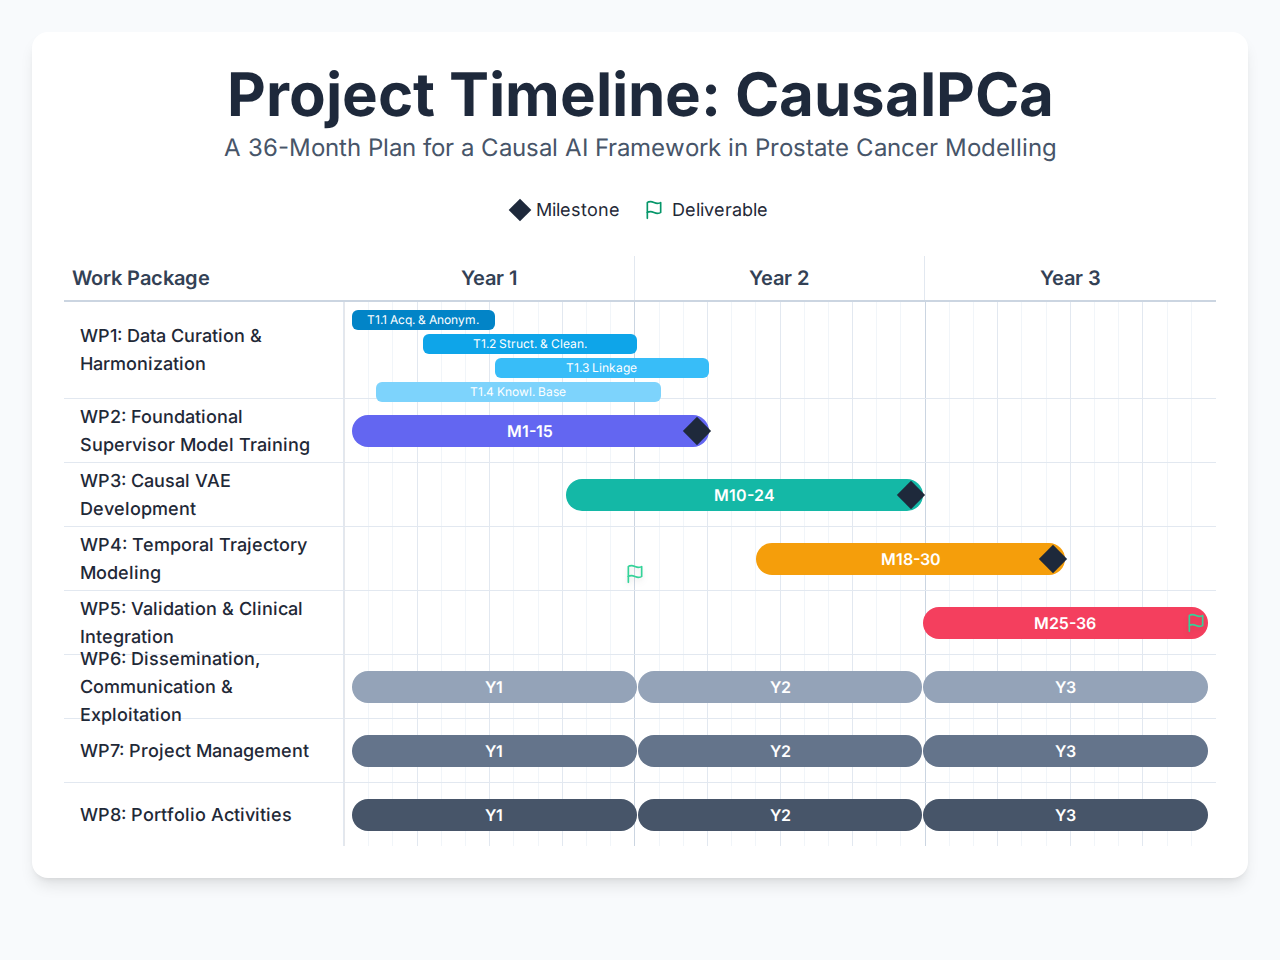
\includegraphics[width=\textwidth]{gantt.png}
    \caption{Project Gantt Chart illustrating the timeline for Work Packages, Deliverables (D), and Milestones (M).}
    \label{fig:gantt}
\end{figure}

\begin{itemize}
    \item \textbf{WP1: Data Curation and Harmonization (30 PMs):} Gather, anonymize, and harmonize multi-modal data.
    \item \textbf{WP2: Foundational Supervisor Model Training (50 PMs):} Develop supervisor models for clinical ground truth.
    \item \textbf{WP3: Causal VAE Development (60 PMs):} Develop the hierarchical \gls{vae} for disentanglement.
    \item \textbf{WP4: Temporal Trajectory Modeling (60 PMs):} Develop the \gls{njde} framework for longitudinal modeling.
    \item \textbf{WP5: Validation and Clinical Integration (30 PMs):} Evaluate the framework's performance and clinical utility.
    \item \textbf{WP6: Dissemination, Communication, and Exploitation (10 PMs):} Manage dissemination, communication, and exploitation activities.
    \item \textbf{WP7: Project Management (10 PMs):} Coordinate the project, including administrative and financial management.
    \item \textbf{WP8: Portfolio Activities (10 PMs):} Foster collaboration across the EIC Pathfinder Challenge portfolio.
\end{itemize}

Key deliverables and milestones are defined in Tables~\ref{tab:deliverables} and~\ref{tab:milestones}.

\begin{table}[H]
    \centering
    \caption{List of Project Deliverables.}
    \label{tab:deliverables}
    \small
    \begin{tabular}{lp{5.5cm}lccr}
        \toprule
        \textbf{Del. No.} & \textbf{Deliverable Name} & \textbf{WP} & \textbf{Type} & \textbf{Dissem.} & \textbf{Due} \\
        \midrule
        D1.1 & Curated, harmonized dataset (initial) & WP1 & Data & CO & M12 \\
        D2.1 & Validated supervisor models & WP2 & Code & PU & M15 \\
        D3.1 & Disentangled VAE models & WP3 & Code & PU & M24 \\
        D4.1 & Trained Neural Jump ODE model & WP4 & Code & PU & M30 \\
        D5.1 & Final validation report & WP5 & R & PU & M36 \\
        D6.1 & Project website and open-source repo & WP6 & Web & PU & M3 \\
        D6.2 & Mid-term dissemination report & WP6 & R & PU & M18 \\
        D6.3 & Final dissemination \& exploitation plan & WP6 & R & PU & M36 \\
        D7.1 & Project management handbook & WP7 & R & CO & M2 \\
        D8.1 & Contribution to Portfolio Strategic Plan & WP8 & R & SEN & M6 \\
        D8.2 & Report on portfolio activities (Year 1) & WP8 & R & SEN & M12 \\
        D8.3 & Report on portfolio activities (Year 2) & WP8 & R & SEN & M24 \\
        D8.4 & Report on portfolio activities (Year 3) & WP8 & R & SEN & M36 \\
        \bottomrule
        \multicolumn{6}{p{13cm}}{\footnotesize \textbf{Type:} R=Report, Data=Dataset, Code=Software, Web=Website. \textbf{Dissem:} PU=Public, CO=Confidential, SEN=Sensitive.}
    \end{tabular}
\end{table}

Complementing the deliverables, the project's progress will be assessed against the verifiable milestones listed in Table~\ref{tab:milestones}. These milestones serve as critical checkpoints to validate the achievement of the project's scientific and technical goals.

\begin{table}[H]
    \centering
    \caption{List of Verifiable Milestones.}
    \label{tab:milestones}
    \small
    \begin{tabular}{lp{5.5cm}lcp{5cm}}
        \toprule
        \textbf{MS No.} & \textbf{Milestone Name} & \textbf{WP} & \textbf{Due} & \textbf{Means of Verification} \\
        \midrule
        M1 & Project Kick-off and Risk Register established & WP7 & M1 & Kick-off meeting minutes; Initial Risk Register document available. \\
        M2 & Supervisor models achieve target performance & WP2 & M15 & Validation report showing mean accuracy >0.75 on internal test set. \\
        M3 & VAE models demonstrate successful disentanglement & WP3 & M24 & Report with quantitative disentanglement metrics (measured by reduced mutual information between dimensions of latent space without trained disentanglement) and qualitative results. \\
        M4 & NJDE model successfully predicts patient trajectories & WP4 & M30 & Report on temporal model performance, with mean accuracy >0.75 for predicting TNM and PSA at different time points. \\
        M5 & Final model validated for clinical plausibility & WP5 & M36 & Final validation report where a majority of counterfactual images are deemed plausible and useful by testing physicians. \\
        \bottomrule
    \end{tabular}
\end{table}

\begin{longtable}{p{0.05\textwidth} p{0.25\textwidth} p{0.1\textwidth} p{0.1\textwidth} p{0.4\textwidth}}
    \caption{Critical Risks and Mitigation Strategies.}
    \label{tab:risks} \\
    \toprule
    \textbf{No.} & \textbf{Description} & \textbf{Likelihood} & \textbf{Impact} & \textbf{Mitigation Strategy} \\
    \midrule
    \endfirsthead
    \multicolumn{5}{c}%
    {{\bfseries \tablename\ \thetable{} -- continued from previous page}} \\
    \toprule
    \textbf{No.} & \textbf{Description} & \textbf{Likelihood} & \textbf{Impact} & \textbf{Mitigation Strategy} \\
    \midrule
    \endhead
    \midrule \multicolumn{5}{r}{{Continued on next page}} \\
    \endfoot
    \bottomrule
    \endlastfoot
    1 & Training Instability and Data Scalability & High & High & Implement a sequential, multi-stage training framework to manage model complexity and ensure controlled progression. Employ a modular design to enable isolated testing and troubleshooting of components. Expected effect: Reduce risk of system-wide failure, stabilize training, and facilitate scalable integration across datasets. \\
    \addlinespace
    2 & Generalizability and Overfitting to Spurious Correlations & Medium & High & Principled disentanglement to separate causal factors from confounders. Use of multi-center data and strong inductive biases (e.g., ordinal losses). Compliant with AI Act Articles 10 \& 15. \\
    \addlinespace
    3 & Performance with Incomplete and Heterogeneous Data & High & High & Neural Jump ODE architecture is inherently designed for sparse, irregular data. A masked loss function allows the model to learn from all available data without being penalized for missingness. \\
    \addlinespace
    4 & Clinical Trustworthiness and the "Black Box" Problem & Medium & High & Explainability through counterfactuals allows clinicians to probe model reasoning. System is designed as a decision support tool, ensuring human oversight at all times. Compliant with AI Act Articles 13 \& 14. \\
    \addlinespace
    5 & Model Drift and Performance Deterioration & Medium & High & Grounding the model in fundamental biological knowledge through disentanglement makes it more robust to superficial data shifts. Continuous monitoring will be implemented to detect performance degradation early. \\
\end{longtable}

\subsection{Quality of the Team and Collaborations}
This project is submitted by a single applicant, the Universitätsklinik für Radiologie und Nuklearmedizin, which possesses the requisite multimodal data, a proven track record in AI model development, and the critical clinical expertise to ensure the solution's reliability. While there is no formal consortium, the project is built on a foundation of \textbf{strong, established collaborations} with key clinical partners who will be contributing data and expertise: the \textbf{Department of Nuclear Medicine at University Hospital Halle}, \textbf{Charité - Universitätsmedizin Berlin}, and the \textbf{Radiological Practice Sudenburg}. A medical doctor with dual specialization in nuclear medicine and radiology will serve as the PI, and a medical doctor with a specialization in nuclear medicine and an IT background will act as co-coordinator.

The applicant's team has extensive, demonstrated experience in the core technologies required for this project, including synthetic CT creation from nuclear imaging, clinical decision support systems, and semi-automatic image segmentation pipelines. Our proven expertise in these areas significantly de-risks the technical development and is showcased on our public portfolio website: \url{https://jakubmitura14.github.io/OVGU_nuclear_projects/}.

Our clinic manages the full range of \gls{pca} cases, including mCRPC, and administers a wide array of treatments, including ARPIs, chemotherapies, and RLT. This provides a rich source of high-quality data for training a causal model. A key strength is our experience with $^{177}$Lu-\gls{psma} theranostics, which provides paired diagnostic and therapeutic scans, ideal for modeling treatment response. This deep clinical and technical expertise, combined with our strong collaborative network, uniquely positions us to succeed in this ambitious project.

\subsection{Appropriateness of the Allocation of Resources}
A key strength of this proposal is the direct access to already preprocessed, rich, longitudinal, and multimodal data from the applicant's own clinical institutions and established collaborators as described in Table \ref{tab:data}. This will form the core training dataset, which can be expanded with new cases during the project from our own or collaborating institutions. An ethical approval for using the preprocessed data for scientific purposes has already been obtained.

The proprietary clinical cohort will serve as the cornerstone of this project, providing a rich, real-world dataset that spans the entire disease spectrum. The core data for all patients will consist of advanced imaging modalities (\gls{pet}/\gls{ct}, \gls{mri}, SPECT/\gls{ct}) and clinical data (\gls{ehr}, lab values). From this clinical data, we will experiment with and derive various features that have proven prognostic impact, such as \gls{psadt}, tumor volume, and the number of bone metastases \cite{guidelines_uro_1,guidelines_uro_2}. As an extension to the core dataset, the framework is designed to be augmented with the following data types on an opportunistic basis, when available:

\begin{itemize}
    \item \textbf{Histopathological Images:} When available, \gls{wsi} from biopsy and prostatectomy specimens will be collected to provide ground-truth information on tumor grade and morphology.
    \item \textbf{Omics Data:} The dataset will be enriched, when possible, with genetic data (e.g., from targeted sequencing panels for genes like BRCA1/2) and other omics data, including proteomics and radiomics features extracted from the imaging studies.
\end{itemize}

\begin{table}[H]
\caption{Summary of Data Sources and Cohorts}
\label{tab:data}
\begin{tabular}{p{0.4\textwidth} p{0.4\textwidth} p{0.2\textwidth}}
\toprule
\textbf{Data Type} & \textbf{Contributing Institutions} & \textbf{Min. Patient Count} \\
\midrule
\multicolumn{3}{l}{\textbf{Proprietary Multi-Center Clinical Cohort}} \\
\midrule
Paired $^{68}$Ga-\gls{psma} \gls{pet}/\gls{ct} \& mp\gls{mri} & Magdeburg, Halle, Charite & 350 \\
\cmidrule(lr){1-3}
Paired pre-therapy $^{68}$Ga-\gls{psma} \gls{pet}/\gls{ct} \& post-therapy $^{177}$Lu-\gls{psma} SPECT/\gls{ct} & Magdeburg, Halle, Charite & 550 \\
\cmidrule(lr){1-3}
Paired interim therapy $^{68}$Ga-\gls{psma} \gls{pet}/\gls{ct} \& \gls{ct} & Magdeburg & 40 \\
\cmidrule(lr){1-3}
Longitudinal $^{68}$Ga-\gls{psma} \gls{pet}/\gls{ct} & Magdeburg & 200 \\
\cmidrule(lr){1-3}
Diagnostic \gls{ct} \& mp\gls{mri} & Rad. Sudenburg (Magdeburg) & 200 \\
\midrule
\textbf{Total Minimum Proprietary Cohort} & & \textbf{1340} \\
\midrule
\multicolumn{3}{p{\dimexpr\linewidth-2\tabcolsep}}{\small\textit{Note: The patient counts are minimum estimates and are expected to increase during the project.}} \\
\midrule
\multicolumn{3}{l}{\textbf{Integration with Public Datasets}} \\
\midrule
Genomic, \gls{mri}, \gls{ct}, \gls{pet} Data & \gls{tcga} \cite{zuley2016cancer} & 14 \\
\cmidrule(lr){1-3}
Longitudinal \gls{mri} (297) \& PSA Data & ProstateNET (\gls{eucaim}) \cite{prostateNetArchive} & 297 \\
\bottomrule
\end{tabular}
\end{table}

The total requested budget for the CausalPCa project is \textbf{\EUR{3,339,253}} over a period of 36 months. While this amount is below the indicative EUR 4 million ceiling for EIC Pathfinder Challenges, it is the result of a meticulous and strategic planning process. The budget is not a reflection of reduced ambition, but rather of a lean, efficient project design that leverages significant existing institutional resources, including access to high-quality data and established clinical infrastructure. This allows us to focus EU funding on the most critical, high-risk research and development activities, ensuring that every euro is directed towards achieving the project's transformative goals. We are confident that this well-justified budget is both realistic and sufficient to deliver on all the project's ambitious objectives and to establish a new European standard for trustworthy clinical AI. The costs are broken down by Work Package (WP) and cost category, with detailed justifications provided below. All costs are estimated in EUR.

\subsubsection*{A.1 Personnel Costs}
Personnel costs are the most significant part of the budget, reflecting the highly skilled, interdisciplinary team required for this project. Integrating advanced imaging, clinical data, and multi-omics data requires a diverse team with expertise in nuclear medicine, radiology, data science, mathematics, and software engineering. Costs are calculated for a 36-month project duration based on institutional salary tables (TV-L), including all social security contributions. A total of \textbf{282 person-months (PMs)} are budgeted.

\begin{itemize}
    \item \textbf{Scientific Staff (Wissenschaftlicher Mitarbeiter) - PI (1 FTE, 36 PMs):} \EUR{263,141}
    \item \textbf{Scientific Staff (Wissenschaftlicher Mitarbeiter) - PhD Student (3 FTEs, 108 PMs):} \EUR{789,423}
    \item \textbf{Scientific Staff (Wissenschaftlicher Mitarbeiter) - Mathematician (0.5 FTE, 18 PMs):} \EUR{131,571}
    \item \textbf{Scientific Staff (Wissenschaftlicher Mitarbeiter) - Data Scientist (1 FTE, 36 PMs):} \EUR{263,141}
    \item \textbf{Technical Staff (Technischer Angestellter) - Programmer (2 FTEs, 72 PMs):} \EUR{405,966}
    \item \textbf{Technical Staff (Technischer Angestellter) - Project Manager (0.5 FTE, 18 PMs):} \EUR{101,492}
    \item \textbf{Student/Research Assistant (Wissenschaftliche Hilfskraft) (40hrs/month, 36 months):} \EUR{33,040}
\end{itemize}

\textbf{Total Estimated Personnel Costs: \EUR{1,987,774}}

\paragraph{Personnel Justification}
The personnel budget is structured to support the project's ambitious goals through a dedicated, interdisciplinary team. The roles are defined based on the German academic system (TV-L) and reflect the required level of experience for each position. The justification for each role is as follows:
\begin{itemize}
    \item \textbf{Scientific Staff (Wissenschaftlicher Mitarbeiter) - PI (Senior Researcher, 1 FTE, 36 PMs):} The PI will provide the overall scientific vision and leadership, ensuring the project stays on track and meets its objectives. They will coordinate the complex, interdisciplinary work across all WPs and lead the high-level scientific dissemination and exploitation activities (WP6, WP7). The co-coordinator will support the PI and have defined responsibilities for the technical development and implementation of the AI framework.
    \item \textbf{Scientific Staff (Wissenschaftlicher Mitarbeiter) - PhD Student (Postdoctoral Researcher, 3 FTEs, 108 PMs):} Three PhD students are critical for the project's execution. Their roles are multifaceted, involving the crucial tasks of data curation, cleaning, and annotation across all data modalities, including imaging, histopathology, and omics data. They will also be instrumental in implementing and training the AI models and conducting the rigorous experimental validation needed to ensure their robustness and accuracy. Their work will directly support the clinical teams in urology, nuclear medicine, radiology, and histopathology and will form the foundation of their doctoral theses.
    \item \textbf{Scientific Staff (Wissenschaftlicher Mitarbeiter) - Mathematician (Senior Researcher, 0.5 FTE, 18 PMs):} A half-time mathematician is required to provide the essential theoretical support for the novel causal models being developed. This role will focus on ensuring the mathematical soundness of the framework, particularly the complex Neural Jump ODEs (WP4), and will contribute to the development of robust uncertainty quantification methods.
    \item \textbf{Scientific Staff (Wissenschaftlicher Mitarbeiter) - Data Scientist (Senior Researcher, 1 FTE, 36 PMs):} A dedicated data scientist is vital for managing the project's complex and heterogeneous data. This role will oversee the entire data pipeline, from curation and harmonization (WP1) to secure storage and access, ensuring the integrity and usability of the data for all technical work packages.
    \item \textbf{Technical Staff (Technischer Angestellter) - Programmer (Experienced, 2 FTEs, 72 PMs):} Two full-time programmers are required to build the robust, scalable, and production-ready software that forms the backbone of this project. They will be responsible for the end-to-end software engineering, including developing the data processing pipelines, implementing the AI models with a focus on efficiency and optimization, and creating the user-facing clinical validation tools.
    \item \textbf{Technical Staff (Technischer Angestellter) - Project Manager (Experienced, 0.5 FTE, 18 PMs):} A part-time project manager is essential for the operational success of this multi-partner project. This role extends beyond standard administrative duties to include coordinating data sharing and harmonization between the collaborating clinics, managing the grant documentation and reporting to the EC, and actively tracking development logs to ensure all project activities are compatible with the principles and requirements of the EU AI Act (WP7).
    \item \textbf{Student/Research Assistant (Wissenschaftliche Hilfskraft) (40hrs/month, 36 months):} A part-time research assistant will provide essential support for the data collection efforts and the clinical validation studies in WP5, assisting with patient data management and study logistics.
\end{itemize}

\subsubsection*{A.2 Equipment Costs}
The requested budget for computational resources represents a strategic, one-time capital investment in the core enabling technology of this project. This on-premise infrastructure is not an operational overhead but the central scientific instrument—the \textbf{primary discovery engine}—required to achieve the project's groundbreaking ambition. The amount is based on a detailed analysis of the project's workload and market pricing for state-of-the-art AI hardware. In accordance with EU and national regulations, only the depreciation costs corresponding to the project duration and usage will be budgeted.

\begin{table}[H]
\centering
\caption{The Revised Computational Resource Budget (3 Years)}
\label{tab:computational_budget}
\sisetup{group-separator={,}}
\begin{tabular}{lS[table-format=6.0]S[table-format=6.0]S[table-format=6.0]S[table-format=6.0]}
\toprule
\textbf{Cost Category} & {\textbf{Year 1 (€)}} & {\textbf{Year 2 (€)}} & {\textbf{Year 3 (€)}} & {\textbf{Total (€)}} \\
\midrule
NVIDIA DGX B200 System & 489000 & 0 & 0 & 489000 \\
300 TB Storage Solution & 28000 & 0 & 0 & 28000 \\
Installation \& Integration & 19000 & 0 & 0 & 19000 \\
\midrule
\textbf{TOTAL} & \textbf{536000} & \textbf{0} & \textbf{0} & \textbf{536000} \\
\bottomrule
\end{tabular}
\end{table}

\paragraph{1. Strategic Imperative and Project Relevance}
To pursue the project's visionary goal of creating a causal AI framework for medicine, an investment in computational power commensurate with the scale of the scientific challenge is required. The budget is therefore centered on the acquisition of an \textbf{NVIDIA DGX B200 system}. This is not a conventional server but a purpose-built, integrated AI supercomputer that directly addresses the primary technical risks of the project. The equipment is indispensable for the execution of \textbf{WP2, WP3, and WP4}, which involve training deep learning models on large-scale 3D imaging data.

\paragraph{2. Justification for the DGX B200 Solution}
The choice of the DGX B200 is driven by key technical requirements of the proposed research:
\begin{itemize}
    \item \textbf{Solving the VRAM Bottleneck:} The project's focus on high-resolution 3D medical imaging is severely limited by GPU memory (VRAM). The DGX B200 provides a massive \textbf{1.44 TB of unified, high-bandwidth GPU memory}, which is essential for training the large, complex 3D VAE and Diffusion Models at the heart of our methodology. This capability is critical to de-risk the core of the project.
    \item \textbf{Powering Complex, Multi-Stage Workflows:} Our four-stage causal framework requires intensive, iterative re-training cycles. The DGX B200's architecture, with eight tightly interconnected GPUs, is engineered for exactly this kind of complex, distributed workload, ensuring maximum efficiency for model development.
    \item \textbf{Turnkey Solution to Reduce Engineering Overhead:} As a fully integrated and validated platform, the DGX B200 allows the research team to focus immediately on scientific discovery rather than spending months on system integration and debugging. It includes the necessary NVIDIA AI Enterprise software and support, accelerating the timeline from deployment to discovery.
    \item \textbf{High-Throughput Data Processing:} The system's architecture, including features like GPUDirect Storage, is optimized to handle the large-scale (~200-400 TB) multimodal datasets of this project, ensuring the powerful GPUs are never left "starved" for data.
\end{itemize}

\paragraph{3. Depreciation and Project-Specific Usage}
The total purchase cost of the DGX B200 system, including storage and integration, is estimated at \EUR{536,000}. Following institutional and EU guidelines, we will depreciate the equipment over a standard useful life of 5 years (60 months). As this equipment is being procured specifically for this project and its unique computational demands, it will be dedicated \textbf{100\% to project activities} for its entire 36-month duration within the project. The eligible depreciation cost is therefore calculated as:
$$ (\text{Total Cost} / \text{Useful Life in Months}) \times \text{Project Duration in Months} \times \text{Usage \%} $$
$$ (536,000 / 60) \times 36 \times 1.0 = \text{\EUR{321,600}} $$
Usage will be tracked and documented through the system's job submission and resource allocation logs to ensure a clear and auditable trail of its dedication to the project.

\textbf{Total Estimated Equipment Costs (Eligible Depreciation): \EUR{321,600}}

\subsubsection*{A.3 Travel Costs}
The travel budget is allocated for project meetings and dissemination of project results at leading international conferences.
\begin{itemize}
    \item \textbf{Project Meetings (3):} Budget for travel and accommodation for the project team and key external collaborators to attend a kick-off meeting (M1 in Magdeburg), a mid-term review meeting (M18), and a final project meeting (M36 in Magdeburg).
    \item \textbf{International Conferences (6):} Budget to allow key personnel (PI, PhDs, Programmers) to present project findings at major international conferences such as RSNA, ECR, MICCAI, and NeurIPS. This is crucial for WP6 (Dissemination).
\end{itemize}

\textbf{Total Estimated Travel Costs: \EUR{32,500}}

\subsubsection*{A.4 Other Direct Costs}
This category includes costs for publications, dataset access, and other minor expenses.
\begin{itemize}
    \item \textbf{Open Access Publication Fees:} To comply with Horizon Europe's open science mandate, we have budgeted for Article Processing Charges (APCs) for an estimated 10 high-impact journal publications.
    \item \textbf{UK Biobank Access:} A fee of \EUR{12,000} is budgeted for access to the UK Biobank dataset.
    \item \textbf{Software Licenses:} A provision of \EUR{36,000} is budgeted for specialized software licenses, including for NVIDIA AI Enterprise.
    \item \textbf{Clinical Consultations:} A budget of \EUR{54,000} is allocated for small monthly consultations with external experts in urology, histopathology, and radiology to ensure the project remains clinically relevant.
\end{itemize}

\textbf{Total Estimated Other Direct Costs: \EUR{112,000}}

\subsubsection*{B. Indirect Costs (Overheads)}
Indirect costs are calculated as a flat rate of \textbf{25\% of the total direct costs}, in accordance with EIC Lump Sum rules. These costs cover general institutional overheads.

\textbf{Total Direct Costs (A): \EUR{2,668,274}}

\textbf{Indirect Costs (B = 25\% of A): \EUR{667,069}}

\subsubsection*{C. Total Project Budget}
The total requested funding is the sum of total direct and indirect costs.

\textbf{Total Estimated Project Cost (A + B):} \EUR{3,335,343}

\subsubsection*{Budget Allocation per Work Package (in EUR)}

\begin{table}[H]
\centering
\caption{Estimated Budget Allocation per Work Package}
\label{tab:budget_wp}
\sisetup{group-separator={,}}
\begin{tabular}{lS[table-format=7.0]S[table-format=6.0]S[table-format=7.0]}
\toprule
\textbf{Work Package} & {\textbf{Direct Costs}} & {\textbf{Indirect Costs}} & {\textbf{Total Cost}} \\
\midrule
WP1: Data Curation & 450000 & 112500 & 562500 \\
WP2: Supervisor Models & 523000 & 130750 & 653750 \\
WP3: Causal VAE & 583000 & 145750 & 728750 \\
WP4: Temporal Modeling & 523000 & 130750 & 653750 \\
WP5: Validation & 200000 & 50000 & 250000 \\
WP6: Dissemination & 110000 & 27500 & 137500 \\
WP7: Project Management & 279274 & 69819 & 349093 \\
\midrule
\textbf{Total} & {\textbf{2668274}} & {\textbf{667069}} & {\textbf{3335343}} \\
\bottomrule
\end{tabular}
\end{table}

\subsection{Compliance and Portfolio Contribution}
This combined data strategy provides an unparalleled foundation for this high-risk, high-gain project, mitigating the risk of data scarcity and ensuring the developed technology is robust, validated, and ready for broader clinical application.

\textbf{Data Governance, AI Act Compliance (Article 10), and \gls{eucaim} Integration:} All data will be managed within a secure, learning-ready environment based on the XNAT platform, ensuring robust data hosting and management. Our data governance framework is designed to meet the stringent quality criteria of Article 10 of the EU AI Act and to ensure full compatibility with the \gls{eucaim} infrastructure. We commit to making all collected data ready for integration into the \gls{eucaim} federation.

Our strategy for \gls{eucaim} compatibility includes:
\begin{itemize}
    \item \textbf{Contribution Model:} We will operate as a \textbf{Tier 3 Federated Node}. This model preserves our data sovereignty while enabling participation in advanced, privacy-preserving federated learning activities. We commit to providing the necessary local infrastructure and a 95\% \gls{sla} to support this role.
    \item \textbf{Data Harmonization and Interoperability:} All our data will be harmonized and structured according to the \gls{eucaim} \gls{cdm}, which is based on \gls{omopcdm} and \gls{fhir} standards. We will map our local data schema to the \gls{eucaim} hyper-ontology to ensure semantic interoperability.
    \item \textbf{Legal and Ethical Adherence:} We will execute a \gls{dsa} with the \gls{eucaim} consortium. All data processing is covered by approvals from our institutional ethics committee and is fully compliant with the General Data Protection Regulation (\gls{gdpr}) and the German Federal Data Protection Act.
\end{itemize}

The data collection is overseen by our clinical partners, and all data undergoes a rigorous curation and verification process by trained clinicians to ensure it is relevant, representative, and as free of errors as possible. To address potential biases, our disentanglement methods (Stage 2) and confounder models (Stage 1) are designed to detect and mitigate biases related to demographics and acquisition hardware. For the purpose of bias detection and correction, we will process special categories of personal data only where strictly necessary and with the appropriate safeguards as permitted under Article 10(5), ensuring our dataset is suitable for training a high-risk AI system.

The project's success will be measured through a rigorous, multi-faceted evaluation plan that combines quantitative metrics with qualitative, clinician-in-the-loop studies to assess real-world utility and trustworthiness.

\subsubsection{Quantitative Metrics}
Model performance will be assessed using a comprehensive suite of metrics tailored to each sub-task, presented in a clear "Metric - What it measures - Why it's relevant" format:
\begin{itemize}
    \item \textbf{Supervisor Model Performance:}
        \begin{itemize}
            \item \textbf{Classification (Accuracy, \gls{auc}, F1-Score, Quadratic Weighted Kappa):} These metrics measure the model's ability to correctly classify categorical variables like TNM stage and PI-RADS score. They are relevant for assessing the model's fundamental diagnostic accuracy.
            \item \textbf{Survival Regression (\gls{cindex}, \gls{mae}):} These metrics measure the model's ability to predict \gls{ttp}. They are relevant for assessing the model's prognostic accuracy.
        \end{itemize}
    \item \textbf{Generative Model Performance:}
        \begin{itemize}
            \item \textbf{Image Generation Quality (\gls{fid}, \gls{ssim}, \gls{lpips}):} These metrics measure the realism and fidelity of the generated images. They are relevant for ensuring the clinical plausibility of the model's outputs.
            \item \textbf{Counterfactual Quality (Axiomatic Soundness, Validity):} These metrics assess the logical consistency and effectiveness of the generated counterfactuals. They are relevant for ensuring the trustworthiness and explainability of the model.
        \end{itemize}
\end{itemize}

\subsubsection{Uncertainty Quantification}
A key feature for clinical trust is the model's ability to quantify its own uncertainty. Our \gls{vae}-based architecture is intrinsically probabilistic and allows for robust uncertainty quantification. We will employ two complementary methods:
\begin{itemize}
    \item \textbf{Latent Space Sampling:} For a given input, we will draw multiple samples from its learned latent distribution. The variance in the resulting predictions will serve as a robust measure of the model's epistemic uncertainty \cite{BustinMeyer2025}.
    \item \textbf{Direct Variance Utilisation:} The variance vector $\sigma^2$ produced by the \gls{vae} encoder is a direct indicator of feature-level uncertainty. We will concatenate this variance vector to the mean vector as a direct input to downstream models, allowing them to learn to depend more on high-confidence features \cite{FriedrichFrisch2024}.
\end{itemize}

\subsubsection{Component-Wise and Joint Validation Strategy}
Our validation strategy is designed to rigorously test each component of the framework in isolation before assessing the performance of the integrated system. This staged approach, detailed in Table \ref{tab:validation_strategy}, ensures that each module is robust and reliable before it is incorporated into the full clinical workflow.

\begin{table}[H]
    \centering
    \caption{Component-Wise and Joint Validation Strategy.}
    \label{tab:validation_strategy}
    \small
    \begin{tabular}{p{0.25\textwidth} p{0.35\textwidth} p{0.35\textwidth}}
        \toprule
        \textbf{Component/Stage} & \textbf{Isolated Testing} & \textbf{Joint Testing} \\
        \midrule
        \textbf{Stage 1: Supervisor Models} & Each model (ordinal classifiers, survival regressor, etc.) will be tested independently against its specific ground truth using standard metrics (Accuracy, AUC, C-index). & The outputs of the supervisor models will be used as inputs for the VAEs in Stage 2. The quality of the VAE's disentanglement will serve as an indirect measure of the supervisor models' performance. \\
        \addlinespace
        \textbf{Stage 2: Causal VAEs} & The VAEs will be evaluated on their ability to generate realistic images (measured by FID, SSIM) and to successfully disentangle the latent space (measured by mutual information metrics). & The disentangled latent vectors from the VAEs will be used as inputs for the NJDE model in Stage 3. The NJDE's predictive accuracy will be used to assess the quality of the learned representations. \\
        \addlinespace
        \textbf{Stage 3: Neural Jump ODE} & The NJDE will be tested on its ability to accurately predict future latent states from a given history, using a masked loss function to handle missing data. & The predicted latent states from the NJDE will be passed to the VAE decoders to generate future images. The quality of these generated images will be assessed both quantitatively (FID, SSIM) and qualitatively by clinicians. \\
        \addlinespace
        \textbf{Stage 4: Full Framework} & The complete, end-to-end framework will be evaluated in a simulated clinical environment. This includes testing the user interface and the generation of structured reports. & A comprehensive clinical plausibility and workflow integration study will be conducted, as detailed below, to assess the real-world utility and trustworthiness of the full system. \\
        \bottomrule
    \end{tabular}
\end{table}

\subsubsection{Clinical Plausibility and Workflow Integration Study}
Beyond quantitative metrics, a practical, clinician-in-the-loop study is essential to assess the model's real-world utility and trustworthiness.
\begin{itemize}
    \item \textbf{Assessing Counterfactual Plausibility and Usefulness:} To evaluate the quality of our generated explanations, we will conduct a human-grounded study with radiologists and oncologists. Clinicians will be presented with a series of cases, each including an original image and its corresponding model-generated counterfactual (e.g., an image of a tumorous prostate and its benign-looking counterfactual). They will score the counterfactuals on a Likert scale for:
    \begin{itemize}
        \item \textbf{Clinical Plausibility:} Does the generated image appear realistic and anatomically sound?
        \item \textbf{Usefulness for Explanation:} Does the visual difference between the original and counterfactual image provide a clear and understandable reason for the model's prediction?
    \end{itemize}
    \item \textbf{Measuring Workflow Improvement with Structured Reports:} To assess the impact of the automated reports, we will perform a comparative workflow study. A control group of clinicians will review patient cases using traditional free-text reports and standard image viewers. An experimental group will review the same cases using our system's auto-generated structured reports and prognostic visualizations. We will measure:
    \begin{itemize}
        \item \textbf{Efficiency:} Time taken to extract key information (e.g., TNM stage, PI-RADS score, presence of key findings) required for treatment planning.
        \item \textbf{Accuracy and Concordance:} Inter-rater agreement and accuracy of the extracted information compared to an expert-defined ground truth.
        \item \textbf{User Satisfaction:} Clinicians' perceived efficiency, clarity, and confidence in their decisions will be assessed using a standardized questionnaire (e.g., the System Usability Scale).
    \end{itemize}
\end{itemize}

Furthermore, comprehensive \textbf{technical documentation} will be maintained throughout the project as specified in Annex IV of the AI Act, and our system's design includes automatic logging capabilities to ensure traceability of operations, in compliance with the record-keeping requirements of \textbf{Articles 11 and 12}.
\subsection{Compliance with the EU Artificial Intelligence Act}
The proposed framework is designed from the ground up to align with the principles of trustworthy AI and to comply with the requirements for high-risk AI systems as laid down in the Regulation (EU) 2024/1689 (the "AI Act"). As a system intended for use in medical diagnosis and to guide treatment, it is classified as a \textbf{high-risk AI system} under Annex III of the Act. Our methodology directly addresses the core obligations for such systems:

\begin{itemize}
    \item \textbf{Risk Management System (Article 9):} Our project management (WP7) will implement a continuous, iterative risk management process as mandated by Article 9, which will be maintained throughout the AI system’s lifecycle. Specifically, this will be operationalized through a dedicated \textbf{Risk Register}, established at the project's outset (M1). This living document will log all known and reasonably foreseeable risks to health, safety, fundamental rights, and project execution. For each identified risk, we will assess its severity and likelihood, and define concrete mitigation and contingency plans. The register will be reviewed quarterly by the project management team and discussed in detail during biannual project meetings with the external collaborators. The applicant (Universitätsklinik für Nuklearmedizin, Magdeburg) will take the lead in identifying clinical risks (e.g., misdiagnosis, incorrect treatment suggestions), while the technical team will focus on system-level risks (e.g., model bias, cybersecurity vulnerabilities, performance degradation). This structured and collaborative process ensures that risks are not only identified but actively managed and mitigated throughout the project.

    \item \textbf{Data and Data Governance (Article 10):} WP1 is entirely dedicated to establishing data governance practices that meet the quality criteria of Article 10. We will use relevant, representative datasets. We will proactively implement measures to detect and mitigate potential biases through the disentanglement methods in Stage 2 and the confounder models in Stage 1. While sex as a biological variable is fixed for prostate cancer, the project will also investigate and mitigate potential data biases related to other demographic factors (e.g., age, ethnicity) to ensure the model's equity and generalizability. For the purpose of bias detection and correction, we will process special categories of personal data only where strictly necessary and with the appropriate safeguards as permitted under Article 10(5).

    \item \textbf{Technical Documentation and Record-Keeping (Articles 11 \& 12):} We commit to creating and maintaining comprehensive technical documentation as specified in Annex IV of the AI Act. Our system's design includes automatic logging capabilities to ensure traceability of operations, in compliance with the record-keeping requirements of Article 12.

    \item \textbf{Transparency and Provision of Information (Article 13):} A cornerstone of our project is to overcome the "black box" problem. The framework's ability to generate counterfactual explanations (Stage 4) is a direct implementation of the transparency requirements of Article 13. The system is designed so that its operations are sufficiently transparent to enable deployers to interpret its output and use it appropriately. We will provide detailed instructions for use that explain the system's capabilities, limitations, and the role of human oversight.

    \item \textbf{Human Oversight (Article 14):} The system is designed to augment, not replace, clinical experts. It functions as a decision support tool, ensuring that a natural person can oversee its functioning at all times. The design ensures that the user can understand the system's capabilities, monitor its operation, and decide to disregard, override, or reverse its output, fulfilling the requirements of Article 14.

    \item \textbf{Accuracy, Robustness, and Cybersecurity (Article 15):} WP5 is dedicated to rigorous validation of the model's accuracy and robustness. The system will be designed to be resilient against errors and inconsistencies through the disentanglement of confounders (Stage 2). To comply with Article 15, we will implement a multi-layered, comprehensive security strategy that addresses AI-specific threats, ensures patient data privacy, and enforces strict regulatory compliance \cite{AlAttar2023,AlkanZakariyya2025}. Our approach is built on three pillars:

\paragraph{1. Enhancing AI Model Robustness and Integrity}
To defend against malicious inputs and training manipulations, we will:
\begin{itemize}
    \item \textbf{Stress Testing and OOD Detection:} We will conduct rigorous stress tests to validate robustness and implement \gls{ood} detection to flag inputs that fall outside the model's expected data range, thereby preserving reliability \cite{KhadkaEpiphaniou2025}.
    \item \textbf{Data Quality Assessment:} We will perform thorough checks on all data for completeness, consistency, and correctness to avoid performance degradation \cite{GarcaGmezBlanesSelva2023}.
\end{itemize}

\paragraph{2. Operational, Transparency, and Regulatory Frameworks}
To ensure accountability and long-term reliability, we will establish:
\begin{itemize}
    \item \textbf{Continuous Monitoring and Anomaly Detection:} We will implement continuous monitoring to identify anomalous model behaviors in real-time \cite{AlAttar2023,GarcaGmezBlanesSelva2023}.
    \item \textbf{\gls{xai}:} Our counterfactual explanation system is a core part of our \gls{xai} strategy, providing transparency that is crucial for clinician trust and accountability \cite{GarcaGmezBlanesSelva2023,JamesIjiga2024}.
    \item \textbf{A Comprehensive Audit Trail:} We will maintain a complete audit trail logging all user actions, system access, and predictions to ensure traceability \cite{GarcaGmezBlanesSelva2023,KhadkaEpiphaniou2025}.
\end{itemize}
\end{itemize}

This principled approach ensures that our innovative framework is not only technologically advanced but also safe, trustworthy, and fully compliant with the Union's legal framework for artificial intelligence.

\subsection{Portfolio Mapping}
\begin{table}[H]
    \centering
    \caption{Portfolio Mapping.}
    \label{tab:portfolio_mapping}
    \small
    \begin{tabular}{p{0.4\textwidth} p{0.6\textwidth}}
        \toprule
        \textbf{Category} & \textbf{Value} \\
        \midrule
        Type of Cancer & Prostate Cancer \\
        \midrule
        Clinical Area & Predictive Diagnosis, Personalized Treatment Selection \\
        \midrule
        Technological area & GenAI-based tools for Integrating Multidimensional Multimodal Health Data, Medical Data Augmentation, Medical Knowledge Representation and Integration \\
        \midrule
        Access to Infrastructure, Data, and Ecosystem integration & Access to proprietary clinical data from Universitätsklinik für Radiologie und Nuklearmedizin (Magdeburg), Abteilung für Nuklearmedizin at Universitätsmedizin Halle, Universitätsmedizin Charite, and the Radiological Practice Rad. Sudenburg. Integration with public datasets (TCGA-PRAD, ProstateNET). Collaboration with EIBIR and DICOM. Contribution to EUCAIM. \\
        \bottomrule
    \end{tabular}
\end{table}

\section{Conclusions}
This project represents a bold step towards a new frontier in clinical AI. We propose not an incremental improvement, but a foundational shift from correlational pattern recognition to causal, explainable, and trustworthy artificial intelligence. Our vision is to create a dynamic "digital twin" for prostate cancer that empowers clinicians with a tool that can reason, simulate, and explain—augmenting their expertise and enabling truly personalized medicine.

The CausalPCa framework is designed to tackle the immense complexity of prostate cancer by deconstructing it into manageable, causally-grounded stages. By pioneering novel methods in disentanglement, longitudinal modeling, and counterfactual generation, we will deliver a technology that is not only powerful but also robust, generalizable, and aligned with the highest standards of the EU AI Act.

This high-risk, high-gain endeavor will deliver a transformative tool for oncology, establish a new European standard for trustworthy AI, and provide a versatile, foundational technology with the potential to revolutionize how we understand and treat complex diseases. We are confident that the applicant's team, with its deep interdisciplinary expertise and access to unparalleled clinical data, is perfectly positioned to turn this ambitious vision into a reality, generating profound scientific, clinical, and societal impact for Europe.

\bibliographystyle{unsrt}
\bibliography{bibl}

\printglossary[type=\acronymtype, title=List of Acronyms]

\end{document}